% \begin{figure}[htbp]
%     \centering

%     \begin{subfigure}[t]{0.32\textwidth}
%         \centering
%         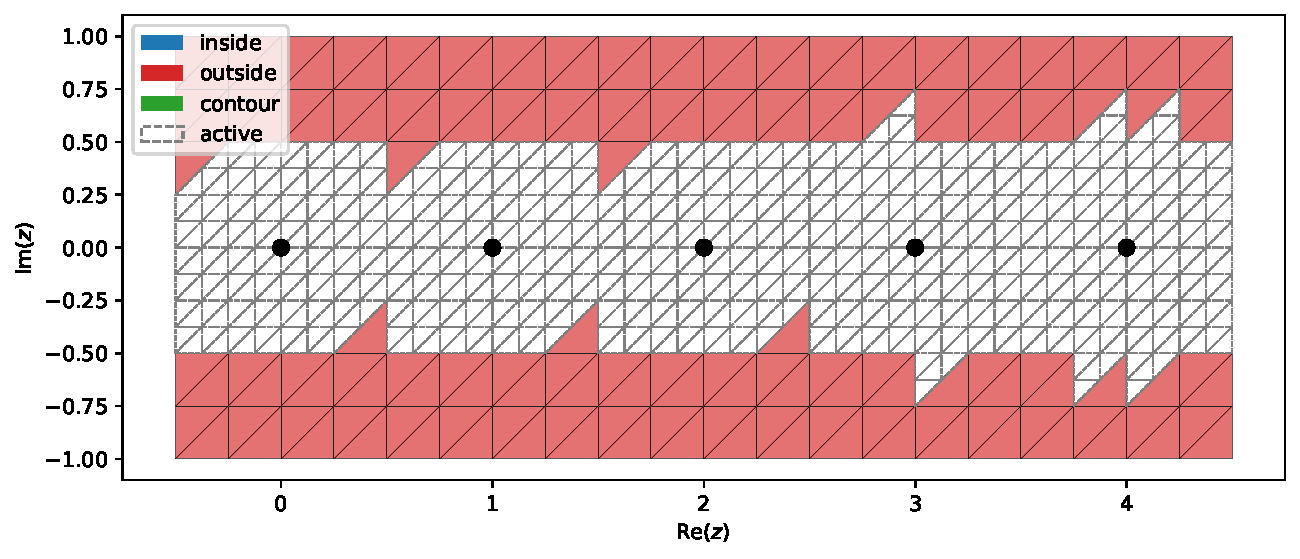
\includegraphics[width=\textwidth]{images/poisson_sweep_000.pdf}
%         \caption{Results for $\mathcal{T}_0.$}
%         \label{fig:dirac-sweep0}
%     \end{subfigure}
%     \hfill
%     \begin{subfigure}[t]{0.32\textwidth}
%         \centering
%         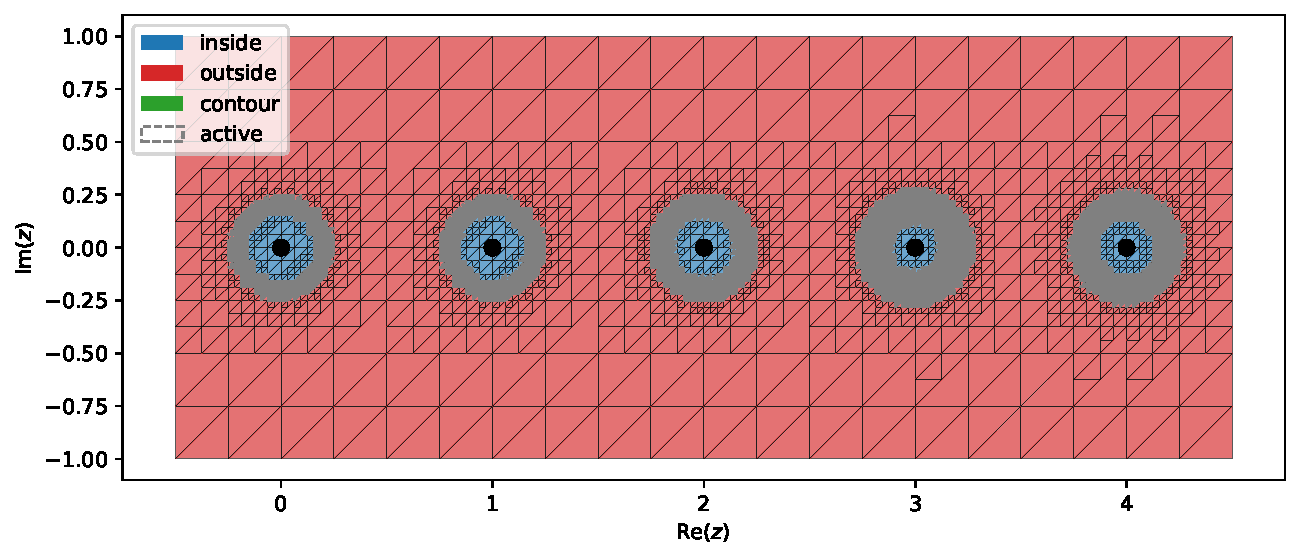
\includegraphics[width=\textwidth]{images/poisson_sweep_003.pdf}
%         \caption{Results for $\mathcal{T}_3.$}
%         \label{fig:dirac-sweep3}
%     \end{subfigure}
%     \hfill
%     \begin{subfigure}[t]{0.32\textwidth}
%         \centering
%         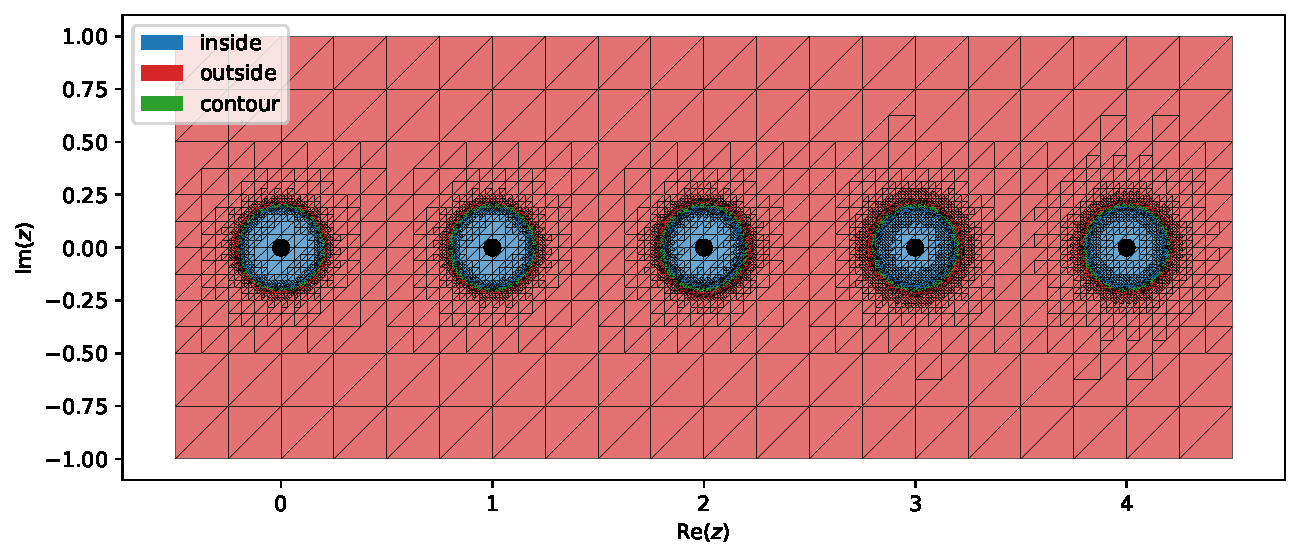
\includegraphics[width=\textwidth]{images/poisson_sweep_006.pdf}
%         \caption{Results for $\mathcal{T}_6.$}
%         \label{fig:dirac-sweep6}
%     \end{subfigure}

%     \caption{Chosen snapshots of Algorithm \ref{outerloop} applied to the $\epsilon = 0.2$ pseudospectrum of \eqref{dirac eig}. The black dots indicate the exact eigenvalues \eqref{eigs dirac}. Red triangles have been classified as outside the $\epsilon$-pseudospectrum, blue triangles have been classified as inside the $\epsilon$-pseudospectrum, green triangles have been classified as lying on the pseudospectral contour, and white triangles outlined in grey remain active. A magnified view of the final result is shown in Figure ?.}
%     \label{dirac results}
% \end{figure}

\begin{figure}[htbp]
    \centering

    \begin{subfigure}[t]{0.8\textwidth}
        \centering
        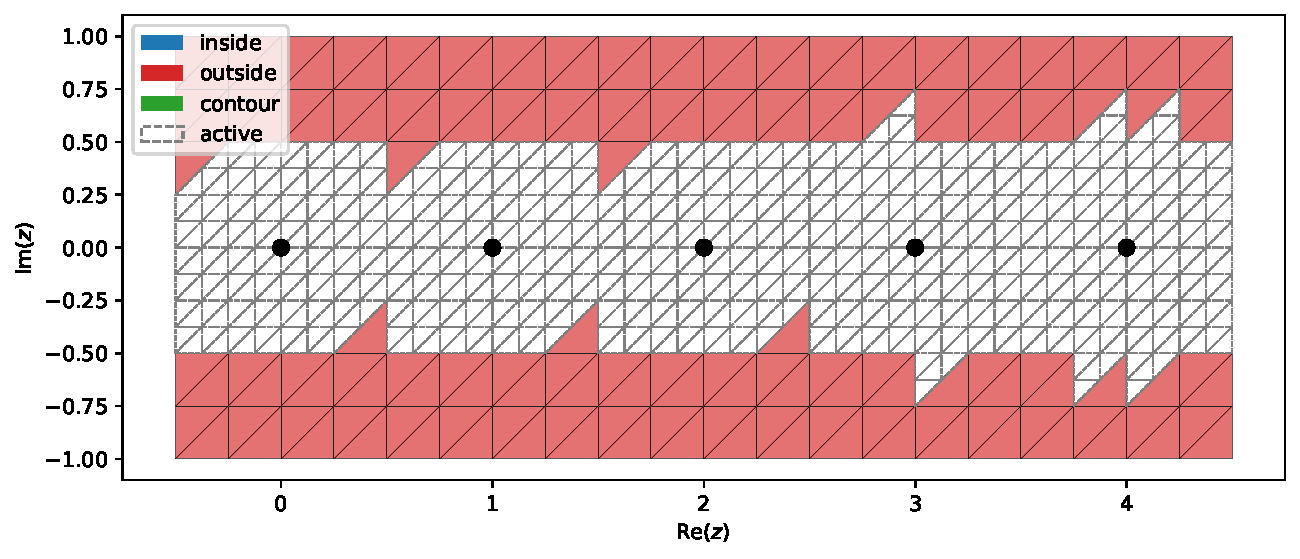
\includegraphics[width=\textwidth]{images/poisson_sweep_000 (1).pdf}
        \caption{Results for $\mathcal{T}_0$.}
        \label{fig:dirac-sweep0}
    \end{subfigure}

    \vspace{0.2em}

    \begin{subfigure}[t]{0.8\textwidth}
        \centering
        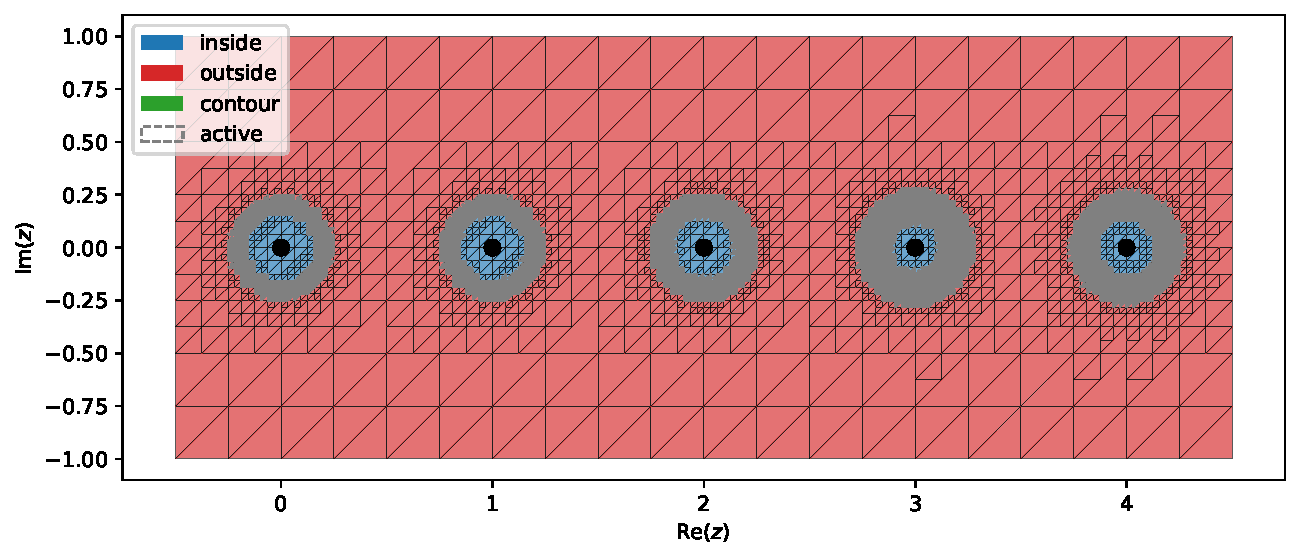
\includegraphics[width=\textwidth]{images/poisson_sweep_003 (1).pdf}
        \caption{Results for $\mathcal{T}_3$.}
        \label{fig:dirac-sweep3}
    \end{subfigure}

    \vspace{0.2em}

    \begin{subfigure}[t]{0.8\textwidth}
        \centering
        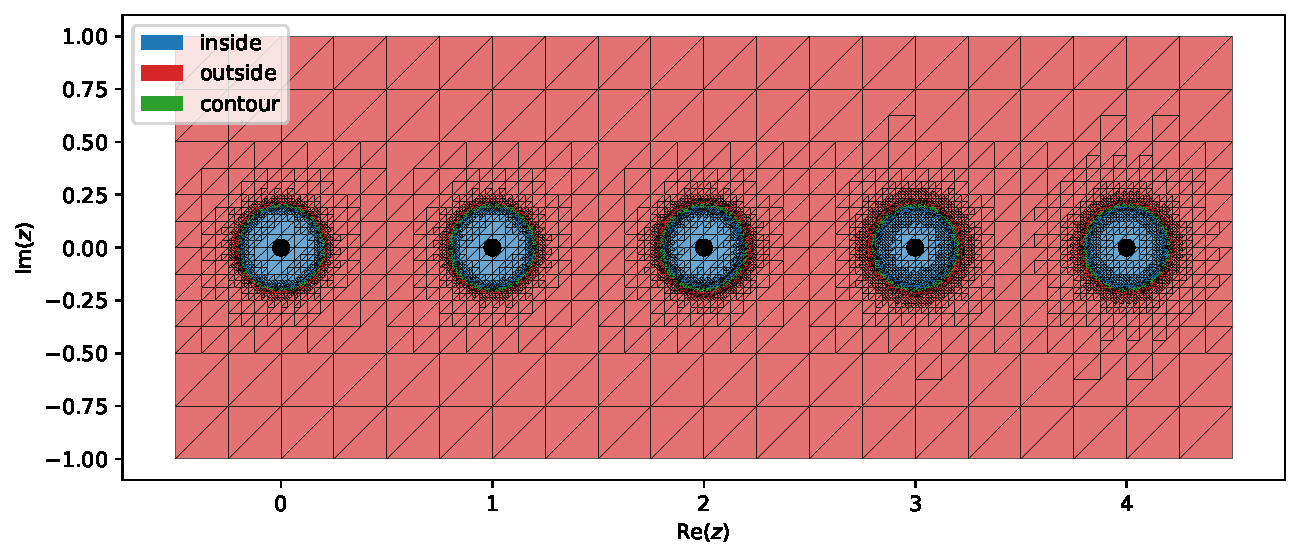
\includegraphics[width=\textwidth]{images/poisson_sweep_006 (1).pdf}
        \caption{Results for $\mathcal{T}_6$.}
        \label{fig:dirac-sweep6}
    \end{subfigure}

    \caption[The Computed $\epsilon = 0.2$ Pseudospectral Picture for the One-Dimensional Dirac-Type Operator.]{Selected snapshots of Algorithm~\ref{outerloop} applied to the
    $\epsilon=0.2$ pseudospectrum of the Diract-type operator \eqref{dirac eig}. The black dots indicate the
    exact eigenvalues \eqref{eigs dirac}. Red triangles have been classified as
    outside the $\epsilon$-pseudospectrum, blue triangles have been classified as inside the $\epsilon$-pseudospectrum, green
    triangles have been classified as lying on the pseudospectral contour, and white triangles
    outlined in grey remain active. The resolution of Figure \ref{fig:dirac-sweep6} makes the green triangles hard to distinguish. We therefore present a magnified view of the final result in Figure~\ref{dirac-zoom}.}
    \label{dirac results}
\end{figure}